\begin{enumerate}[label=\thesubsection.\arabic*.,ref=\thesubsection.\theenumi]
\numberwithin{equation}{enumi}

\item Three identical inverting amplifier stages each characterized by a low frequency gain K and a single pole response with 
\begin{align}
    f_{3dB} = 100kHz
\end{align}
are connected in a feedback loop with H = 1.
What is the minimum value of K at which the circuit oscillates? What would the frequency of oscillation be?\\
\solution
The given data is shown in the table.\ref{table:Input_table}
\begin{table}[!ht]
\centering

%%%%%%%%%%%%%%%%%%%%%%%%%%%%%%%%%%%%%%%%%%%%%%%%%%%%%%%%%%%%%%%%%%%%%%
%%                                                                  %%
%%  This is the header of a LaTeX2e file exported from Gnumeric.    %%
%%                                                                  %%
%%  This file can be compiled as it stands or included in another   %%
%%  LaTeX document. The table is based on the longtable package so  %%
%%  the longtable options (headers, footers...) can be set in the   %%
%%  preamble section below (see PRAMBLE).                           %%
%%                                                                  %%
%%  To include the file in another, the following two lines must be %%
%%  in the including file:                                          %%
%%        \def\inputGnumericTable{}                                 %%
%%  at the beginning of the file and:                               %%
%%        \input{name-of-this-file.tex}                             %%
%%  where the table is to be placed. Note also that the including   %%
%%  file must use the following packages for the table to be        %%
%%  rendered correctly:                                             %%
%%    \usepackage[latin1]{inputenc}                                 %%
%%    \usepackage{color}                                            %%
%%    \usepackage{array}                                            %%
%%    \usepackage{longtable}                                        %%
%%    \usepackage{calc}                                             %%
%%    \usepackage{multirow}                                         %%
%%    \usepackage{hhline}                                           %%
%%    \usepackage{ifthen}                                           %%
%%  optionally (for landscape tables embedded in another document): %%
%%    \usepackage{lscape}                                           %%
%%                                                                  %%
%%%%%%%%%%%%%%%%%%%%%%%%%%%%%%%%%%%%%%%%%%%%%%%%%%%%%%%%%%%%%%%%%%%%%%



%%  This section checks if we are begin input into another file or  %%
%%  the file will be compiled alone. First use a macro taken from   %%
%%  the TeXbook ex 7.7 (suggestion of Han-Wen Nienhuys).            %%
\def\ifundefined#1{\expandafter\ifx\csname#1\endcsname\relax}


%%  Check for the \def token for inputed files. If it is not        %%
%%  defined, the file will be processed as a standalone and the     %%
%%  preamble will be used.                                          %%
\ifundefined{inputGnumericTable}

%%  We must be able to close or not the document at the end.        %%
	\def\gnumericTableEnd{\end{document}}


%%%%%%%%%%%%%%%%%%%%%%%%%%%%%%%%%%%%%%%%%%%%%%%%%%%%%%%%%%%%%%%%%%%%%%
%%                                                                  %%
%%  This is the PREAMBLE. Change these values to get the right      %%
%%  paper size and other niceties.                                  %%
%%                                                                  %%
%%%%%%%%%%%%%%%%%%%%%%%%%%%%%%%%%%%%%%%%%%%%%%%%%%%%%%%%%%%%%%%%%%%%%%

	\documentclass[12pt%
			  %,landscape%
                    ]{report}
       \usepackage[latin1]{inputenc}
       \usepackage{fullpage}
       \usepackage{color}
       \usepackage{array}
       \usepackage{longtable}
       \usepackage{calc}
       \usepackage{multirow}
       \usepackage{hhline}
       \usepackage{ifthen}



%%  End of the preamble for the standalone. The next section is for %%
%%  documents which are included into other LaTeX2e files.          %%
\else

%%  We are not a stand alone document. For a regular table, we will %%
%%  have no preamble and only define the closing to mean nothing.   %%
    \def\gnumericTableEnd{}

%%  If we want landscape mode in an embedded document, comment out  %%
%%  the line above and uncomment the two below. The table will      %%
%%  begin on a new page and run in landscape mode.                  %%
%       \def\gnumericTableEnd{\end{landscape}}
%       \begin{landscape}


%%  End of the else clause for this file being \input.              %%
\fi

%%%%%%%%%%%%%%%%%%%%%%%%%%%%%%%%%%%%%%%%%%%%%%%%%%%%%%%%%%%%%%%%%%%%%%
%%                                                                  %%
%%  The rest is the gnumeric table, except for the closing          %%
%%  statement. Changes below will alter the table's appearance.     %%
%%                                                                  %%
%%%%%%%%%%%%%%%%%%%%%%%%%%%%%%%%%%%%%%%%%%%%%%%%%%%%%%%%%%%%%%%%%%%%%%

\providecommand{\gnumericmathit}[1]{#1} 
%%  Uncomment the next line if you would like your numbers to be in %%
%%  italics if they are italizised in the gnumeric table.           %%
%\renewcommand{\gnumericmathit}[1]{\mathit{#1}}
\providecommand{\gnumericPB}[1]%
{\let\gnumericTemp=\\#1\let\\=\gnumericTemp\hspace{0pt}}
 \ifundefined{gnumericTableWidthDefined}
        \newlength{\gnumericTableWidth}
        \newlength{\gnumericTableWidthComplete}
        \newlength{\gnumericMultiRowLength}
        \global\def\gnumericTableWidthDefined{}
 \fi
%% The following setting protects this code from babel shorthands.  %%
 \ifthenelse{\isundefined{\languageshorthands}}{}{\languageshorthands{english}}
%%  The default table format retains the relative column widths of  %%
%%  gnumeric. They can easily be changed to c, r or l. In that case %%
%%  you may want to comment out the next line and uncomment the one %%
%%  thereafter                                                      %%
\providecommand\gnumbox{\makebox[0pt]}
%%\providecommand\gnumbox[1][]{\makebox}

%% to adjust positions in multirow situations                       %%
\setlength{\bigstrutjot}{\jot}
\setlength{\extrarowheight}{\doublerulesep}

%%  The \setlongtables command keeps column widths the same across  %%
%%  pages. Simply comment out next line for varying column widths.  %%
\setlongtables

\setlength\gnumericTableWidth{%
	53pt+%
	93pt+%
0pt}
\def\gumericNumCols{2}
\setlength\gnumericTableWidthComplete{\gnumericTableWidth+%
         \tabcolsep*\gumericNumCols*2+\arrayrulewidth*\gumericNumCols}
\ifthenelse{\lengthtest{\gnumericTableWidthComplete > \linewidth}}%
         {\def\gnumericScale{\ratio{\linewidth-%
                        \tabcolsep*\gumericNumCols*2-%
                        \arrayrulewidth*\gumericNumCols}%
{\gnumericTableWidth}}}%
{\def\gnumericScale{1}}

%%%%%%%%%%%%%%%%%%%%%%%%%%%%%%%%%%%%%%%%%%%%%%%%%%%%%%%%%%%%%%%%%%%%%%
%%                                                                  %%
%% The following are the widths of the various columns. We are      %%
%% defining them here because then they are easier to change.       %%
%% Depending on the cell formats we may use them more than once.    %%
%%                                                                  %%
%%%%%%%%%%%%%%%%%%%%%%%%%%%%%%%%%%%%%%%%%%%%%%%%%%%%%%%%%%%%%%%%%%%%%%

\ifthenelse{\isundefined{\gnumericColA}}{\newlength{\gnumericColA}}{}\settowidth{\gnumericColA}{\begin{tabular}{@{}p{110pt*\gnumericScale}@{}}x\end{tabular}}
\ifthenelse{\isundefined{\gnumericColB}}{\newlength{\gnumericColB}}{}\settowidth{\gnumericColB}{\begin{tabular}{@{}p{30pt*\gnumericScale}@{}}x\end{tabular}}

\begin{tabular}[c]{%
	b{\gnumericColA}%
	b{\gnumericColB}%
	}

%%%%%%%%%%%%%%%%%%%%%%%%%%%%%%%%%%%%%%%%%%%%%%%%%%%%%%%%%%%%%%%%%%%%%%
%%  The longtable options. (Caption, headers... see Goosens, p.124) %%
%	\caption{The Table Caption.}             \\	%
% \hline	% Across the top of the table.
%%  The rest of these options are table rows which are placed on    %%
%%  the first, last or every page. Use \multicolumn if you want.    %%

%%  Header for the first page.                                      %%
%	\multicolumn{2}{c}{The First Header} \\ \hline 
%	\multicolumn{1}{c}{colTag}	%Column 1
%	&\multicolumn{1}{c}{colTag}	\\ \hline %Last column
%	\endfirsthead

%%  The running header definition.                                  %%
%	\hline
%	\multicolumn{2}{l}{\ldots\small\slshape continued} \\ \hline
%	\multicolumn{1}{c}{colTag}	%Column 1
%	&\multicolumn{1}{c}{colTag}	\\ \hline %Last column
%	\endhead

%%  The running footer definition.                                  %%
%	\hline
%	\multicolumn{2}{r}{\small\slshape continued\ldots} \\
%	\endfoot

%%  The ending footer definition.                                   %%
%	\multicolumn{2}{c}{That's all folks} \\ \hline 
%	\endlastfoot
%%%%%%%%%%%%%%%%%%%%%%%%%%%%%%%%%%%%%%%%%%%%%%%%%%%%%%%%%%%%%%%%%%%%%%

\hhline{|-|-}
	 \multicolumn{1}{|p{\gnumericColA}|}%
	{\gnumericPB{\centering}\gnumbox{\textbf{Parameter}}}
	&\multicolumn{1}{p{\gnumericColB}|}%
	{\gnumericPB{\centering}\gnumbox{\textbf{Value}}}
\\
\hhline{|-|-}
	 \multicolumn{1}{|p{\gnumericColA}|}%
	{\gnumericPB{\centering}\gnumbox{\text{pole frequency}}}
	&\multicolumn{1}{p{\gnumericColB}|}%
	{\gnumericPB{\centering}\gnumbox{\text{100kHz}}}
\\
\hhline{|-|-}
	 \multicolumn{1}{|p{\gnumericColA}|}%
	{\gnumericPB{\centering}\gnumbox{\text{feedback factor}}}
	&\multicolumn{1}{p{\gnumericColB}|}%
	{\gnumericPB{\centering}\gnumbox{\text{1}}}
\\
\hhline{|-|-|}
\end{tabular}

\ifthenelse{\isundefined{\languageshorthands}}{}{\languageshorthands{\languagename}}
\gnumericTableEnd

\caption{INPUT TABLE}
\label{table:Input_table}
\end{table}
\\
The open loop gain of amplifier stages is given by..,
\begin{align}
    G_1(s) = G_2(s) = G_3(s) = \frac{-K}{1+\frac{s}{2\pi10^5}}
\end{align}
The three gains are cascaded.The net open loop gain is given by.,
\begin{align}
    G(s) &= G_1(s)G_2(s)G_3(s)\\
    G(s) &= \sbrak{\frac{-K}{1+\frac{s}{2\pi10^5}}}^3\\
    G(s) &= -\sbrak{\frac{K}{1+\frac{s}{2\pi10^5}}}^3
\end{align}
%------------------------------
\item Draw the control block diagram of above question.\\
\solution 
The control system block is shown in the figure.\ref{fig:control_system}
\begin{figure}[!hbt]
	\begin{center}
			\resizebox{\columnwidth}{!}{\tikzstyle{block} = [draw, fill=blue!20, rectangle, 
    minimum height=3em, minimum width=4em]
\tikzstyle{sum} = [draw, fill=blue!20, circle, node distance=1cm]
\tikzstyle{input} = [coordinate]
\tikzstyle{output} = [coordinate]
\tikzstyle{pinstyle} = [pin edge={to-,thin,black}]


\begin{tikzpicture}[auto, node distance=2cm]
    \node [input, name=input] {};
    \node [sum, right of=input] (sum) {};
    \node [block, right of=sum] (controller1) {$G_1(s)$};
    \node [block, right of=controller1] (controller2) {$G_1(s)$};
    \node [block, right of=controller2] (controller3) {$G_1(s)$};
    \node [output, right of=controller3] (output) {};
    \node [block, below of=controller2] (feedback) {$H = 1$};

    \draw [->] (sum) -- node {$V_i$} (controller1);
    \draw [->] (controller1) -- node {} (controller2);
    \draw [->] (controller2) -- node {} (controller3);
    \draw [->] (controller3) -- node [name=y] {$V_o$}(output);
    \draw [->] (y) |- (feedback);
    \draw [->] (feedback) -| node[pos=0.99]{$-$}  node [near end] {$V_f$} (sum);
\end{tikzpicture}
}
	\end{center}
\caption{CONTROL SYSTEM BLOCK}
\label{fig:control_system}
\end{figure}
%--------------------------------
\item Find the loop gain of the system.\\
\solution The loop gain is given by 
\begin{align}
    LG(s) &= G(s)H \\
    LG(s) &= -\sbrak{\frac{K}{1+\frac{s}{2\pi10^5}}}^3\\
\text{Substitute..,} s=j\omega \\
LG(j\omega) &= -\sbrak{\frac{K}{1+\frac{j\omega}{2\pi10^5}}}^3 \label{eq:ee18btech11031_Transfer_Func}
\end{align}

%-----------------------------------
\item Find the frequency of oscillation of above circuit.\\
\solution According to BarkHausen's criteria..,
\begin{itemize}
    \item The magnitude of loop gain of the system at the oscillating frequency should be greater than or equal to 1.
    \item The phase angle of loop gain at the oscillating frequency must be equal to -180 degrees.
\end{itemize}
Let the frequency of oscillation is fs.,
\begin{align}
    \angle LG(j\omega) = -180\degree\\
    -180\degree - 3tan^{-1}\sbrak{\frac{\omega_s}{2\pi10^5}} = -180\degree \\
    - 3tan^{-1}\sbrak{\frac{\omega_s}{2\pi10^5}} = -360\degree\\
    \frac{\omega_s}{2\pi10^5} =  \tan(120\degree)\\
    \implies \omega_s = 1.088\times10^6\text{ rad/sec}\label{eq:ee18btech11031_frequency}
\end{align}
Thus,the frequency of oscillation is 1.088M rad/sec.
%-----------------------------------
\item Find the minimum value of K.\\
\solution 
We know the magnitude of loop gain is greater than or equal to 1.The range of K can be found as follows,
\begin{align}
    \abs{LG(j\omega_s)} &\geq 1 \\
    \frac{K^3}{\abs{1+\frac{j\omega_s}{2\pi10^5}}^3} &\geq 1 \\
    K^3 &\geq \abs{1+\frac{j1.088\times10^6}{2\pi10^5}}^3\\
     K^3 &\geq \abs{1+j1.73}^3\\
     K^3 &\geq 8 \\
     K &\geq 2
\end{align}
Therefore, The minimum value of K is 2.
%---------------------------------
\item Design the three stage oscillator for the above given question.
\\
\solution Consider the circuit shown in the figure.\ref{fig:ee18btech11031_circuit_design}.\\
\begin{figure}[!hbt]
	\begin{center}
			\resizebox{\columnwidth}{!}{ \begin{circuitikz}
\ctikzset{bipoles/length=1cm}

\draw 
(0, 0) node[op amp] (opamp) {}
(4.5, -0.35) node[op amp] (opamp2) {}
(9, -0.7) node[op amp] (opamp3) {}
(opamp.-) -- (-1,0.35) -- (-1.5,0.35) to[R=$R$] (-3,0.35){}
(-1,0.35)-- (-1,1) to[R=$R_f$] (1.5,1) -- (1.5,0){}
(-1,1) -- (-1,2) to[C= $C$] (1.5,2) -- (1.5,1){}
(1.5,0)--(2,0) to[R=$R$] (3,0)--(3.5,0)--(opamp2.-){}
(opamp2.+)--(3.5,-0.7) node[ground]{}
(opamp.out)--(1.5,0){}
(opamp.+) -- (-1,-0.35) node[ground]{}
(3.5,0) -- (3.5,0.75) to[R=$R_f$] (6,0.75) -- (6,-0.35){}
(3.5,0.75)--(3.5,1.75) to[C=$C$] (6,1.75)--(6,0.35){}
(opamp2.out) -- (6,-0.35){}
(6,-0.35)--(6.5,-0.35) to[R=$R$] (7.5,-0.35)--(8,-0.35)--(opamp3.-){}
(opamp3.+)--(8,-1.05) node[ground]{}
(8,-0.35) -- (8,0.4) to[R=$R_f$] (10,0.4) -- (10,-0.7){}
(8,0.4)--(8,1.4) to[C=$C$] (10,1.4) --(10,0.4){}
(opamp3.out) -- (10,-0.7){}
(10,-0.7) -- (11,-0.7)
(10,-0.7) -- (10,-3)--(-3,-3) -- (-3,0.35){}
node at (-1,0.2){A}
node at (3.5,-0.2){B}
node at (8,-0.7) {C}

node at (1.5,-0.4){$V_1$}
node at (6,-0.6){$V_2$}
node at (11,-1) {$V_{out}$}


;\end{circuitikz}
}
	\end{center}
\caption{1}
\label{fig:ee18btech11031_circuit_design}
\end{figure}
Considering the first stage.,
\begin{align}
    \frac{V_1}{V_{out}} &= -\frac{R_f||\frac{1}{sC}}{R}\\
    \frac{V_1}{V_{out}} &= -\frac{\frac{R_f}{R}}{1+sCR_f}
\end{align}
Similarly for second stage.,
\begin{align}
     \frac{V_2}{V_1} &= -\frac{\frac{R_f}{R}}{1+sCR_f}
\end{align}
Similarly For third stage.,
\begin{align}
     \frac{V_{out}}{V_2} &= -\frac{\frac{R_f}{R}}{1+sCR_f}
\end{align}
Loop gain of the oscillator is computed as follows.,
\begin{align}
    LG(s) &= \frac{V_1}{V_{out}}\times \frac{V_2}{V_1}\times \frac{V_{out}}{V_2} \\
    LG(s) &= \sbrak{-\frac{\frac{R_f}{R}}{1+sCR_f}}^3
\end{align}
Comparing with the equation.\ref{eq:ee18btech11031_Transfer_Func}
\begin{align}
    \frac{R_f}{R} &= K\\
    CR_f &= \frac{1}{2\pi10^5}
\end{align}
For the circuit to oscillate,
\begin{align}
  K \geq 2 \\
  R_f \geq 2R
\end{align}
Choose 
\begin{align}
    R &= 1000\Omega\\
    \implies R_f &= 2000\Omega\\
    \implies C &= 7.9577\times 10^{-10}F
\end{align}
\begin{table}[!ht]
\centering

%%%%%%%%%%%%%%%%%%%%%%%%%%%%%%%%%%%%%%%%%%%%%%%%%%%%%%%%%%%%%%%%%%%%%%
%%                                                                  %%
%%  This is the header of a LaTeX2e file exported from Gnumeric.    %%
%%                                                                  %%
%%  This file can be compiled as it stands or included in another   %%
%%  LaTeX document. The table is based on the longtable package so  %%
%%  the longtable options (headers, footers...) can be set in the   %%
%%  preamble section below (see PRAMBLE).                           %%
%%                                                                  %%
%%  To include the file in another, the following two lines must be %%
%%  in the including file:                                          %%
%%        \def\inputGnumericTable{}                                 %%
%%  at the beginning of the file and:                               %%
%%        \input{name-of-this-file.tex}                             %%
%%  where the table is to be placed. Note also that the including   %%
%%  file must use the following packages for the table to be        %%
%%  rendered correctly:                                             %%
%%    \usepackage[latin1]{inputenc}                                 %%
%%    \usepackage{color}                                            %%
%%    \usepackage{array}                                            %%
%%    \usepackage{longtable}                                        %%
%%    \usepackage{calc}                                             %%
%%    \usepackage{multirow}                                         %%
%%    \usepackage{hhline}                                           %%
%%    \usepackage{ifthen}                                           %%
%%  optionally (for landscape tables embedded in another document): %%
%%    \usepackage{lscape}                                           %%
%%                                                                  %%
%%%%%%%%%%%%%%%%%%%%%%%%%%%%%%%%%%%%%%%%%%%%%%%%%%%%%%%%%%%%%%%%%%%%%%



%%  This section checks if we are begin input into another file or  %%
%%  the file will be compiled alone. First use a macro taken from   %%
%%  the TeXbook ex 7.7 (suggestion of Han-Wen Nienhuys).            %%
\def\ifundefined#1{\expandafter\ifx\csname#1\endcsname\relax}


%%  Check for the \def token for inputed files. If it is not        %%
%%  defined, the file will be processed as a standalone and the     %%
%%  preamble will be used.                                          %%
\ifundefined{inputGnumericTable}

%%  We must be able to close or not the document at the end.        %%
	\def\gnumericTableEnd{\end{document}}


%%%%%%%%%%%%%%%%%%%%%%%%%%%%%%%%%%%%%%%%%%%%%%%%%%%%%%%%%%%%%%%%%%%%%%
%%                                                                  %%
%%  This is the PREAMBLE. Change these values to get the right      %%
%%  paper size and other niceties.                                  %%
%%                                                                  %%
%%%%%%%%%%%%%%%%%%%%%%%%%%%%%%%%%%%%%%%%%%%%%%%%%%%%%%%%%%%%%%%%%%%%%%

	\documentclass[12pt%
			  %,landscape%
                    ]{report}
       \usepackage[latin1]{inputenc}
       \usepackage{fullpage}
       \usepackage{color}
       \usepackage{array}
       \usepackage{longtable}
       \usepackage{calc}
       \usepackage{multirow}
       \usepackage{hhline}
       \usepackage{ifthen}



%%  End of the preamble for the standalone. The next section is for %%
%%  documents which are included into other LaTeX2e files.          %%
\else

%%  We are not a stand alone document. For a regular table, we will %%
%%  have no preamble and only define the closing to mean nothing.   %%
    \def\gnumericTableEnd{}

%%  If we want landscape mode in an embedded document, comment out  %%
%%  the line above and uncomment the two below. The table will      %%
%%  begin on a new page and run in landscape mode.                  %%
%       \def\gnumericTableEnd{\end{landscape}}
%       \begin{landscape}


%%  End of the else clause for this file being \input.              %%
\fi

%%%%%%%%%%%%%%%%%%%%%%%%%%%%%%%%%%%%%%%%%%%%%%%%%%%%%%%%%%%%%%%%%%%%%%
%%                                                                  %%
%%  The rest is the gnumeric table, except for the closing          %%
%%  statement. Changes below will alter the table's appearance.     %%
%%                                                                  %%
%%%%%%%%%%%%%%%%%%%%%%%%%%%%%%%%%%%%%%%%%%%%%%%%%%%%%%%%%%%%%%%%%%%%%%

\providecommand{\gnumericmathit}[1]{#1} 
%%  Uncomment the next line if you would like your numbers to be in %%
%%  italics if they are italizised in the gnumeric table.           %%
%\renewcommand{\gnumericmathit}[1]{\mathit{#1}}
\providecommand{\gnumericPB}[1]%
{\let\gnumericTemp=\\#1\let\\=\gnumericTemp\hspace{0pt}}
 \ifundefined{gnumericTableWidthDefined}
        \newlength{\gnumericTableWidth}
        \newlength{\gnumericTableWidthComplete}
        \newlength{\gnumericMultiRowLength}
        \global\def\gnumericTableWidthDefined{}
 \fi
%% The following setting protects this code from babel shorthands.  %%
 \ifthenelse{\isundefined{\languageshorthands}}{}{\languageshorthands{english}}
%%  The default table format retains the relative column widths of  %%
%%  gnumeric. They can easily be changed to c, r or l. In that case %%
%%  you may want to comment out the next line and uncomment the one %%
%%  thereafter                                                      %%
\providecommand\gnumbox{\makebox[0pt]}
%%\providecommand\gnumbox[1][]{\makebox}

%% to adjust positions in multirow situations                       %%
\setlength{\bigstrutjot}{\jot}
\setlength{\extrarowheight}{\doublerulesep}

%%  The \setlongtables command keeps column widths the same across  %%
%%  pages. Simply comment out next line for varying column widths.  %%
\setlongtables

\setlength\gnumericTableWidth{%
	53pt+%
	93pt+%
0pt}
\def\gumericNumCols{2}
\setlength\gnumericTableWidthComplete{\gnumericTableWidth+%
         \tabcolsep*\gumericNumCols*2+\arrayrulewidth*\gumericNumCols}
\ifthenelse{\lengthtest{\gnumericTableWidthComplete > \linewidth}}%
         {\def\gnumericScale{\ratio{\linewidth-%
                        \tabcolsep*\gumericNumCols*2-%
                        \arrayrulewidth*\gumericNumCols}%
{\gnumericTableWidth}}}%
{\def\gnumericScale{1}}

%%%%%%%%%%%%%%%%%%%%%%%%%%%%%%%%%%%%%%%%%%%%%%%%%%%%%%%%%%%%%%%%%%%%%%
%%                                                                  %%
%% The following are the widths of the various columns. We are      %%
%% defining them here because then they are easier to change.       %%
%% Depending on the cell formats we may use them more than once.    %%
%%                                                                  %%
%%%%%%%%%%%%%%%%%%%%%%%%%%%%%%%%%%%%%%%%%%%%%%%%%%%%%%%%%%%%%%%%%%%%%%

\ifthenelse{\isundefined{\gnumericColA}}{\newlength{\gnumericColA}}{}\settowidth{\gnumericColA}{\begin{tabular}{@{}p{60pt*\gnumericScale}@{}}x\end{tabular}}
\ifthenelse{\isundefined{\gnumericColB}}{\newlength{\gnumericColB}}{}\settowidth{\gnumericColB}{\begin{tabular}{@{}p{60pt*\gnumericScale}@{}}x\end{tabular}}

\begin{tabular}[c]{%
	b{\gnumericColA}%
	b{\gnumericColB}%
	}

%%%%%%%%%%%%%%%%%%%%%%%%%%%%%%%%%%%%%%%%%%%%%%%%%%%%%%%%%%%%%%%%%%%%%%
%%  The longtable options. (Caption, headers... see Goosens, p.124) %%
%	\caption{The Table Caption.}             \\	%
% \hline	% Across the top of the table.
%%  The rest of these options are table rows which are placed on    %%
%%  the first, last or every page. Use \multicolumn if you want.    %%

%%  Header for the first page.                                      %%
%	\multicolumn{2}{c}{The First Header} \\ \hline 
%	\multicolumn{1}{c}{colTag}	%Column 1
%	&\multicolumn{1}{c}{colTag}	\\ \hline %Last column
%	\endfirsthead

%%  The running header definition.                                  %%
%	\hline
%	\multicolumn{2}{l}{\ldots\small\slshape continued} \\ \hline
%	\multicolumn{1}{c}{colTag}	%Column 1
%	&\multicolumn{1}{c}{colTag}	\\ \hline %Last column
%	\endhead

%%  The running footer definition.                                  %%
%	\hline
%	\multicolumn{2}{r}{\small\slshape continued\ldots} \\
%	\endfoot

%%  The ending footer definition.                                   %%
%	\multicolumn{2}{c}{That's all folks} \\ \hline 
%	\endlastfoot
%%%%%%%%%%%%%%%%%%%%%%%%%%%%%%%%%%%%%%%%%%%%%%%%%%%%%%%%%%%%%%%%%%%%%%

\hhline{|-|-}
	 \multicolumn{1}{|p{\gnumericColA}|}%
	{\gnumericPB{\centering}\gnumbox{\textbf{Parameter}}}
	&\multicolumn{1}{p{\gnumericColB}|}%
	{\gnumericPB{\centering}\gnumbox{\textbf{Value}}}
\\
\hhline{|-|-}
	 \multicolumn{1}{|p{\gnumericColA}|}%
	{\gnumericPB{\centering}\gnumbox{\text{$R$}}}
	&\multicolumn{1}{p{\gnumericColB}|}%
	{\gnumericPB{\centering}\gnumbox{\text{$1000\Omega$}}}
\\
\hhline{|-|-}
	 \multicolumn{1}{|p{\gnumericColA}|}%
	{\gnumericPB{\centering}\gnumbox{\text{$R_f$}}}
	&\multicolumn{1}{p{\gnumericColB}|}%
	{\gnumericPB{\centering}\gnumbox{\text{$2000\Omega$}}}
\\
\hhline{|-|-}
	 \multicolumn{1}{|p{\gnumericColA}|}%
	{\gnumericPB{\centering}\gnumbox{\text{$C$}}}
	&\multicolumn{1}{p{\gnumericColB}|}%
	{\gnumericPB{\centering}\gnumbox{\text{$7.9577\times10^{-10}$}}}
\\
\hhline{|-|-|}
\end{tabular}

\ifthenelse{\isundefined{\languageshorthands}}{}{\languageshorthands{\languagename}}
\gnumericTableEnd

\caption{}
\label{table:Output_table}
\end{table}
%-------------------------
\item Verify the above result using the ngspice simulation.\\
\solution
Follow the instructions of the following README file.
\begin{lstlisting}
spice/ee18btech11031/README
\end{lstlisting}
Connect the circuit shown in fig.\ref{fig:ee18btech11031_circuit_design}:1 in ngspice.
The following netlist file is connected accordingly
\begin{lstlisting}
spice/ee18btech11031/gvv_ngspice.net
\end{lstlisting}
This  netlist file results in a sinusoidal wave with particular frequency.
The following code generates the graph shown in fig.\ref{fig:ee18btech11031_spice1}
\begin{lstlisting}
spice/ee18btech11031/ee18btech11031_ngspice.py
\end{lstlisting}
\begin{figure}[!ht]
\centering
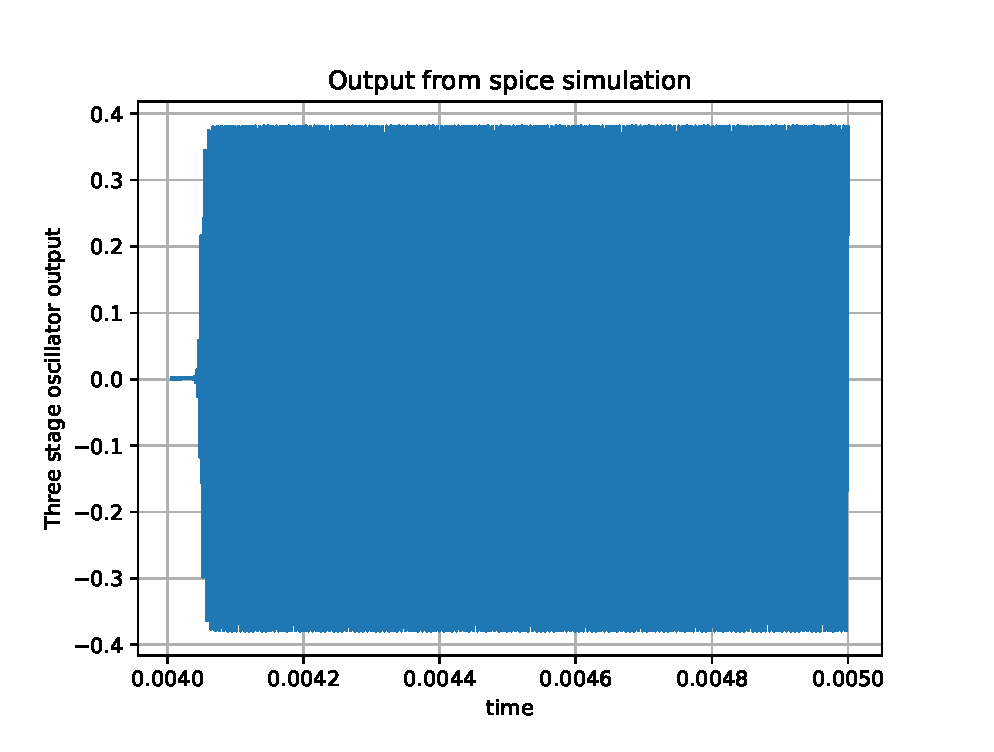
\includegraphics[width=\columnwidth]{./figs/ee18btech11031/ee18btech11031_spice_1.eps}
\caption{Output of three stage oscillator}
\label{fig:ee18btech11031_spice1}
\end{figure}
%------------------
\item Find the frequency of sinusoid obtained from the simulation.\\
\solution The following Netlist file is to generate the output from 4.22msec to 4.26msec
\begin{lstlisting}
spice/ee18btech11031/gvv_ngspice2.net
\end{lstlisting}
The following code generates the variation of output voltage with respect to time.\\
\begin{lstlisting}
spice/ee18btech11031/ee18btech11031_ngspice_2.py
\end{lstlisting}
The data obtained from the above netlist file is plotted in the figure.\ref{fig:ee18btech11031_spice2}.
\begin{figure}[!ht]
\centering
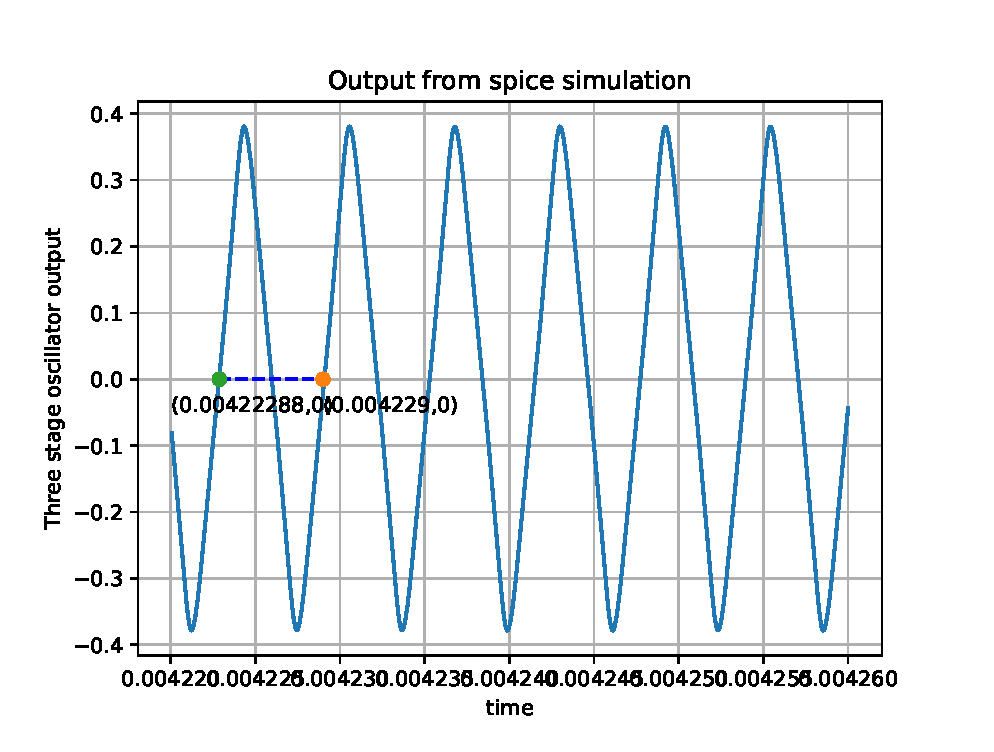
\includegraphics[width=\columnwidth]{./figs/ee18btech11031/ee18btech11031_spice_2.eps}
\caption{Output of three stage oscillator}
\label{fig:ee18btech11031_spice2}
\end{figure}
The frequency obtained in simulation is as follows.,
 \begin{align}
     T_s(spice) &= 4.229\times10^{-3} - 4.2228\times10^{-3}\\
     T_s(spice) &= 6.2\times10^{-6}\\
     \implies F_s(spice) &= 0.1612 \text{MHz}\\
     \implies \omega_s(spice) &= 1.012 \text{ Mrad/sec}
 \end{align}
But the obtained value in equation.\ref{eq:ee18btech11031_frequency} is 1.088MHz.
Thus, the frequency obtained in the spice simulation is approximately equal to the calculated frequency.
\end{enumerate}

